\documentclass[12pt,titlepage]{article}
\usepackage[margin=1.25in]{geometry}
\usepackage{graphicx,amsmath,blindtext,minted}

%% Variables definition
\newcommand{\vSubject}{Web Design and Development}
\newcommand{\vSubtitle}{PHP02}
\newcommand{\vName}{Muhammad Baihaqi Aulia Asy'ari}
\newcommand{\vNIM}{2241720145}
\newcommand{\vClass}{2I}
\newcommand{\vDepartment}{Information Technology}
\newcommand{\vStudyProgram}{D4 Informatics Engineering}

%% [START] Tikz related stuff
\usepackage{tikz}
\usetikzlibrary{svg.path,calc,shapes.geometric,shapes.misc}
\tikzstyle{terminator} = [rectangle, draw, text centered, rounded corners = 1em, minimum height=2em]
\tikzstyle{preparation} = [chamfered rectangle, chamfered rectangle sep=0.75em, draw, text centered, minimum height = 2em]
\tikzstyle{process} = [rectangle, draw, text centered, minimum height=2em]
\tikzstyle{decision} = [diamond, aspect=2, draw, text centered, minimum height=2em]
\tikzstyle{data}=[trapezium, draw, text centered, trapezium left angle=60, trapezium right angle=120, minimum height=2em]
\tikzstyle{connector} = [line width=0.25mm,->]
%% [END] Tikz related stuff

%% [START] Fancy header related stuff
\usepackage{fancyhdr}
\pagestyle{fancy}
\setlength{\headheight}{15pt} % compensate fancyhdr style
\fancyhead{}
\fancyfoot{}
\fancyfoot[L]{\thepage}
\fancyfoot[R]{\textit{\vSubject - \vSubtitle}}
\renewcommand{\footrulewidth}{0.4pt}% default is 0pt, overline for footer
%% [END] Fancy header related stuff

%% [START] Custom tabular command related stuff
\usepackage{tabularx}
\newcommand{\details}[2]{
    #1 & #2  \\
}
%% [END] Custom tabular command related stuff

%% [START] Figure related stuff
\newcommand{\image}[3][1]{
    \begin{figure}[h]
        \centering
        \includegraphics[#1]{#2}
        \caption{#3}
        \label{#3}
    \end{figure}
}
%% [END] Figure related stuff

%%
\usepackage{pgf-umlcd}

\renewcommand{\umldrawcolor}{black}
\renewcommand{\umlfillcolor}{white}
%%

%% [BEGIN] Custom enumerator
\usepackage{enumitem}
%% [END] Custom enumerator

%% [BEGIN] Paragraph indent
\usepackage{indentfirst}
%% [END] Paragraph indent

\begin{document}
\begin{titlepage}
    \centering
    \vfill
    {\bfseries\LARGE
        \vSubject\\
        \vskip0.25cm
        \vSubtitle
    }
    \vfill
    
\includegraphics[width=6cm]{images/polinema-logo.png}
    \vfill
    {
        \textbf{Name}\\
        \vName\\
        \vskip0.5cm
        \textbf{NIM}\\
        \vNIM\\
        \vskip0.5cm
        \textbf{Class}\\
        \vClass\\
        \vskip0.5cm
        \textbf{Department}\\
        \vDepartment\\
        \vskip0.5cm
        \textbf{Study Program}\\
        \vStudyProgram
    }
\end{titlepage}

\newpage

\begin{enumerate}
    \item -
    \begin{minted}[autogobble,breaklines]{html}
        <!-- // ! Experiment 1 - Indexed Array -->
        <!DOCTYPE html>
        <html>
            <head>
            </head>
            <body>
                <h2>Indexed Array</h2>
                <?php
                $listLecturer = ["Alpha", "Bravo", "Charlie"];
        
                // echo $listLecturer[2] . "<br>";
                // echo $listLecturer[0] . "<br>";
                // echo $listLecturer[1] . "<br>";
                
                // looping method
                for ($i=0; $i < sizeof($listLecturer); $i++) { 
                    echo $listLecturer[$i] . "<br>";
                }
                ?>
            </body>
        </html>
    \end{minted}
    \includegraphics[width=.9\textwidth]{images/figures/fig1.png}
    
    \newpage
    
    \item -
    \begin{minted}[autogobble,breaklines]{html}        
        <!-- // ! Experiment 2 - Associative Array -->
        <!DOCTYPE html>
        <html lang="en">
        <head>
            <meta charset="UTF-8">
            <meta name="viewport" content="width=device-width, initial-scale=1.0">
            <title></title>
            <style>
                html {
                    border: 3px solid black;
                }
                table, th, td {
                    border: 1px solid black;
                    border-collapse: collapse;
                }
            </style>
        </head>
        <body>
            <table>
                <tr>
                    <th>Property</th>
                    <th>Value</th>
                </tr>
                <?php
                $lecturer = [
                    'name' => 'Alpha',
                    'domicile' => 'Home',
                    'gender' => 'is a gamelan instrument'
                ];

                // manual
                // echo "Name : {$lecturer['name']} <br>";
                // echo "Domicile : {$lecturer['domicile']} <br>";
                // echo "Gender : {$lecturer['gender']} <br>";

                // looping method
                foreach ($lecturer as $key => $item) {
                    echo "<tr>";
                    echo "<td>{$key}</td>";
                    echo "<td>{$item}</td>";
                    echo "</tr>";
                }
                ?>
            </table>
        </body>
        </html>
    \end{minted}
    \includegraphics[width=.9\textwidth]{images/figures/fig2.png}
    \item - \\ 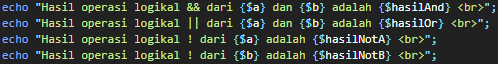
\includegraphics[width=.9\textwidth]{images/figures/fig3.png} \\ You can access multidimentional array with n-dinmension amount of index.
    
    \newpage
    
    \item - \\ \includegraphics[width=.9\textwidth]{images/figures/fig4.png} \\ A function can be use to execute a sequence of code at will
    \item - \\ 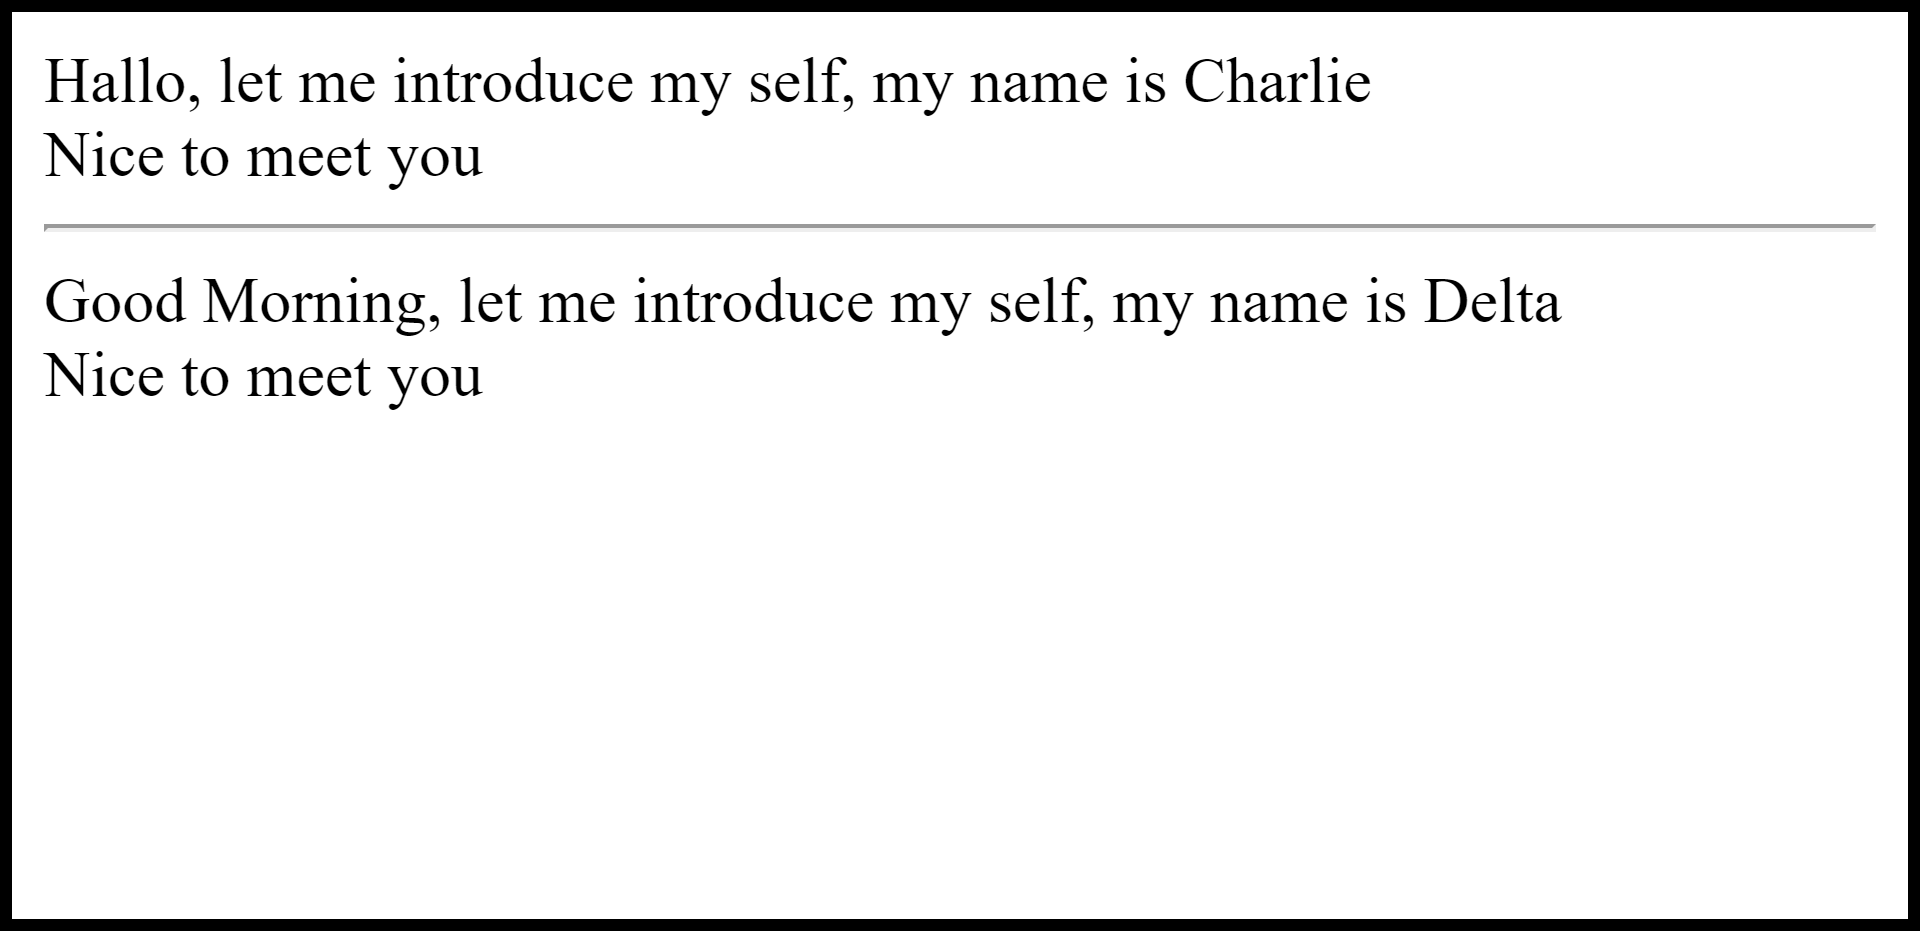
\includegraphics[width=.9\textwidth]{images/figures/fig5.png} \\ You can use a parameter as a variable to be use inside the function. When the function gets called, you can pass the parameter directly or pass it through a variable
    
    \newpage

    \item - \\ 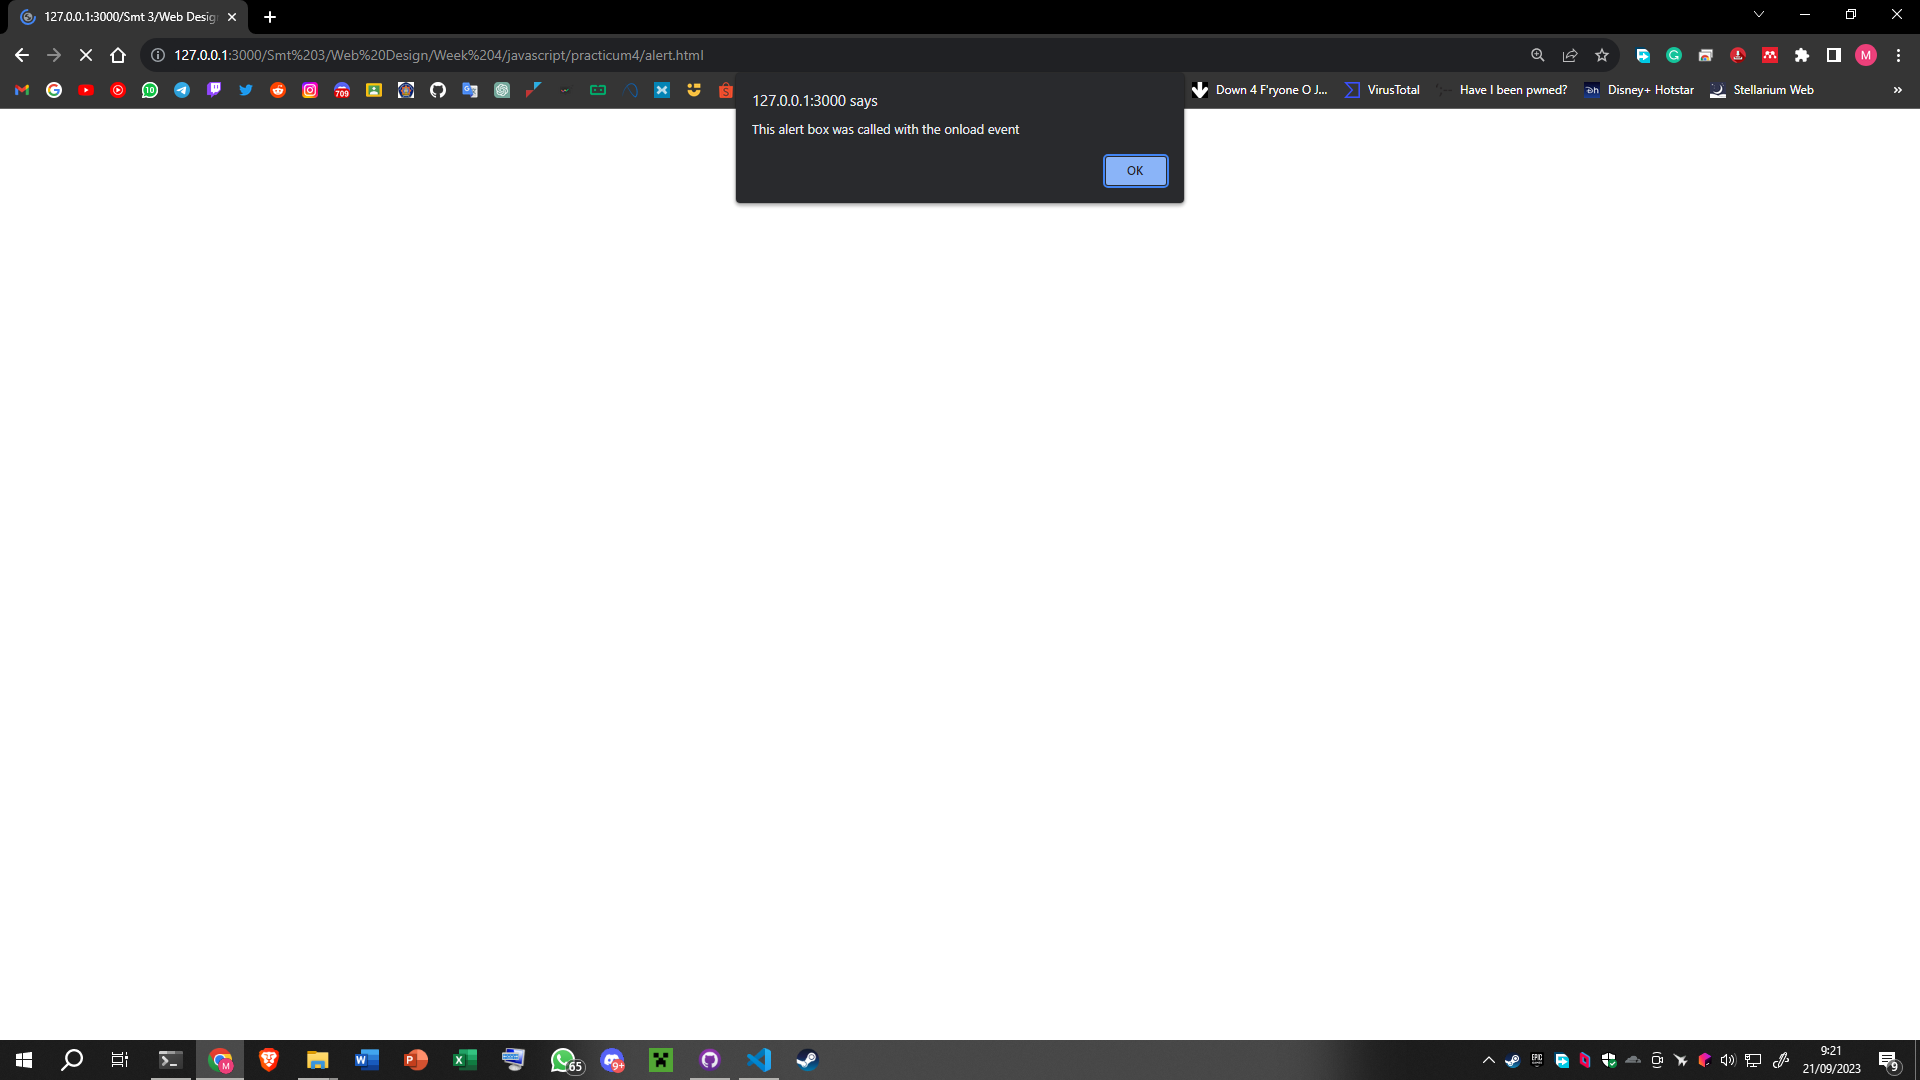
\includegraphics[width=.9\textwidth]{images/figures/fig6.png} \\ Same as before, the only diffrence is that if the function call doesnt inlcude the greetings parameter, it will use the default value set by the function declaration 
    \item - \\ \includegraphics[width=.9\textwidth]{images/figures/fig7.png} \\ The result of the function can be used by calling the function
    
    \newpage
    
    \item - \\ \includegraphics[width=.9\textwidth]{images/figures/fig8.png} \\ The introduction function can use the return value from calculateAge function
    \item - \\ 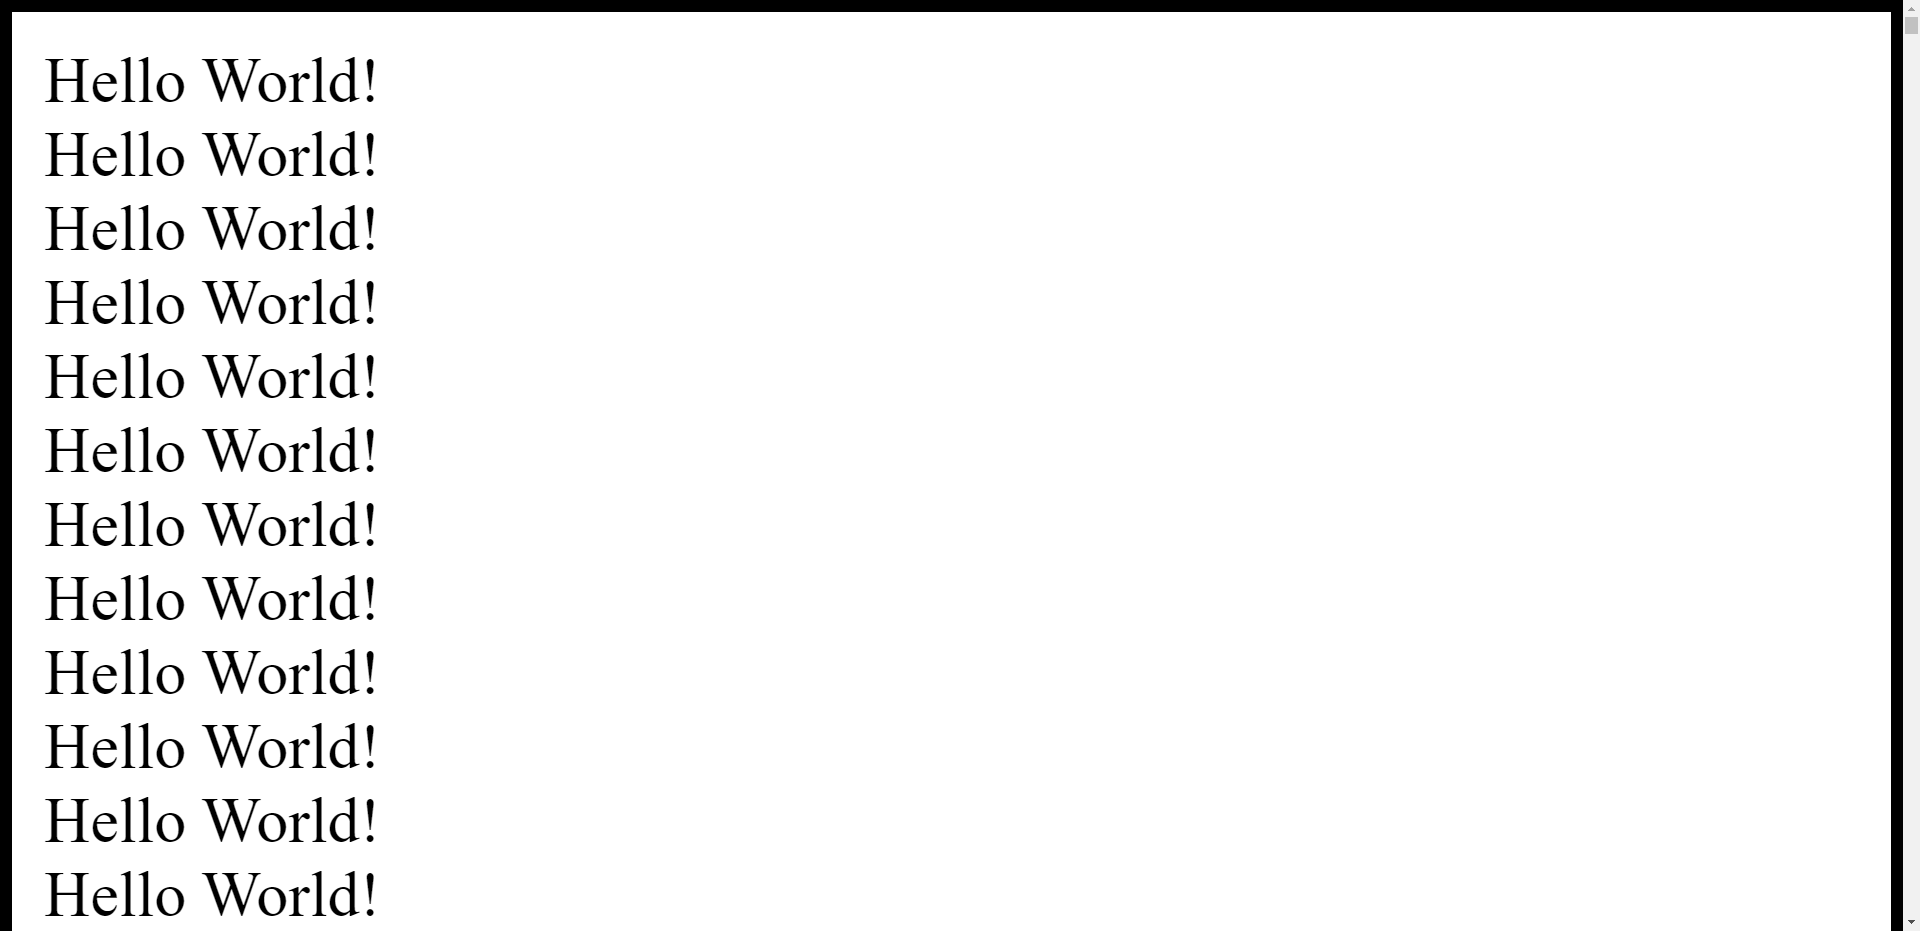
\includegraphics[width=.9\textwidth]{images/figures/fig9.png} \\ The function print the text non-stop
    
    \newpage

    \item - \\ 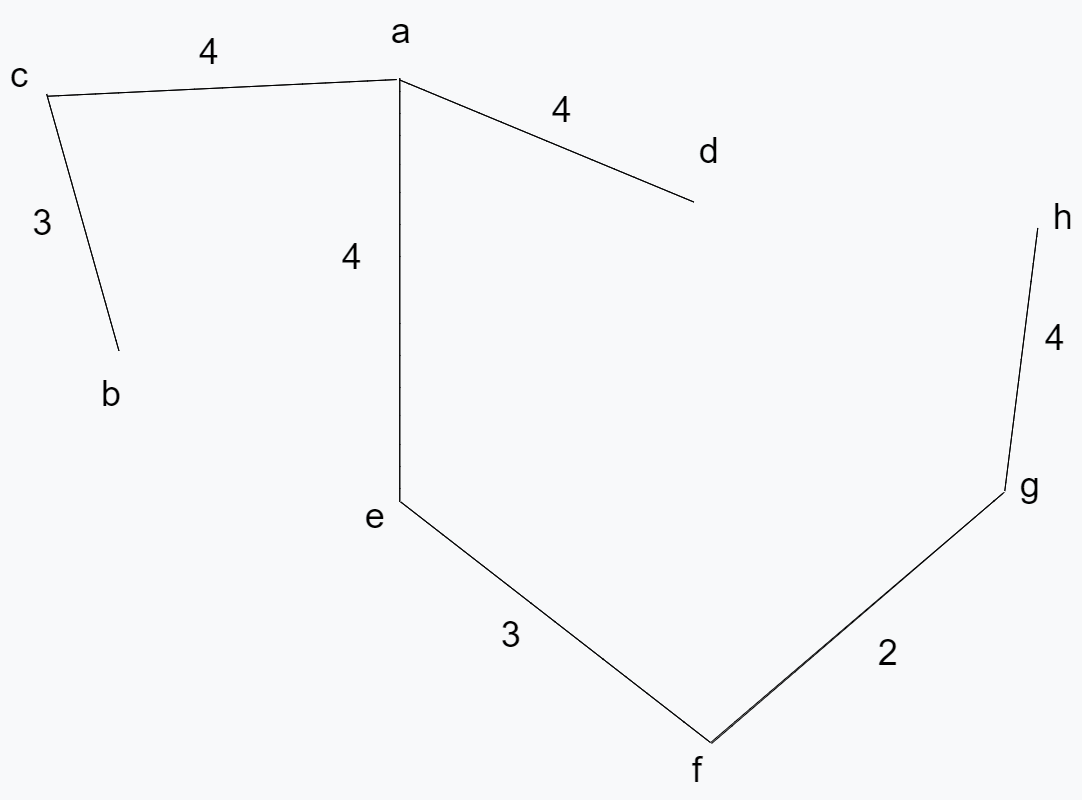
\includegraphics[width=.9\textwidth]{images/figures/fig10.png} \\ The function print the text as long as the index is less than the amount by calling itself and increasing the index in the next function call
    \item - \\ 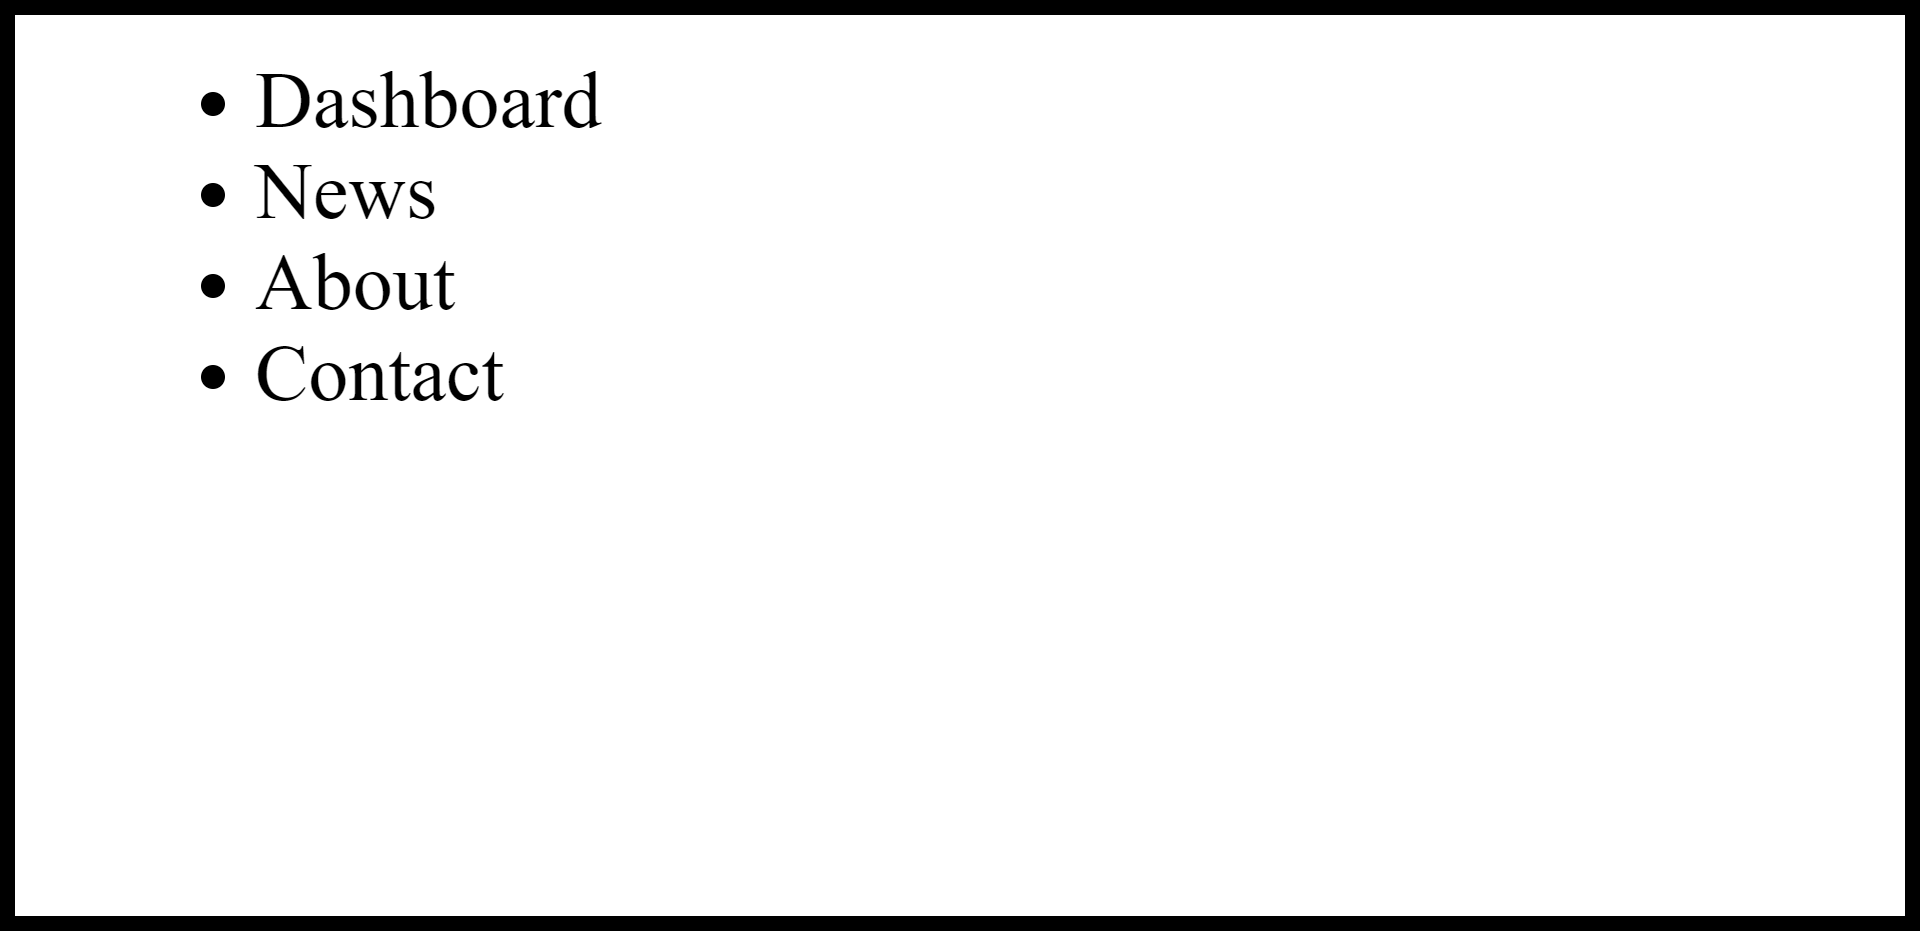
\includegraphics[width=.9\textwidth]{images/figures/fig11.png}
    
    \newpage

    \item - \\ 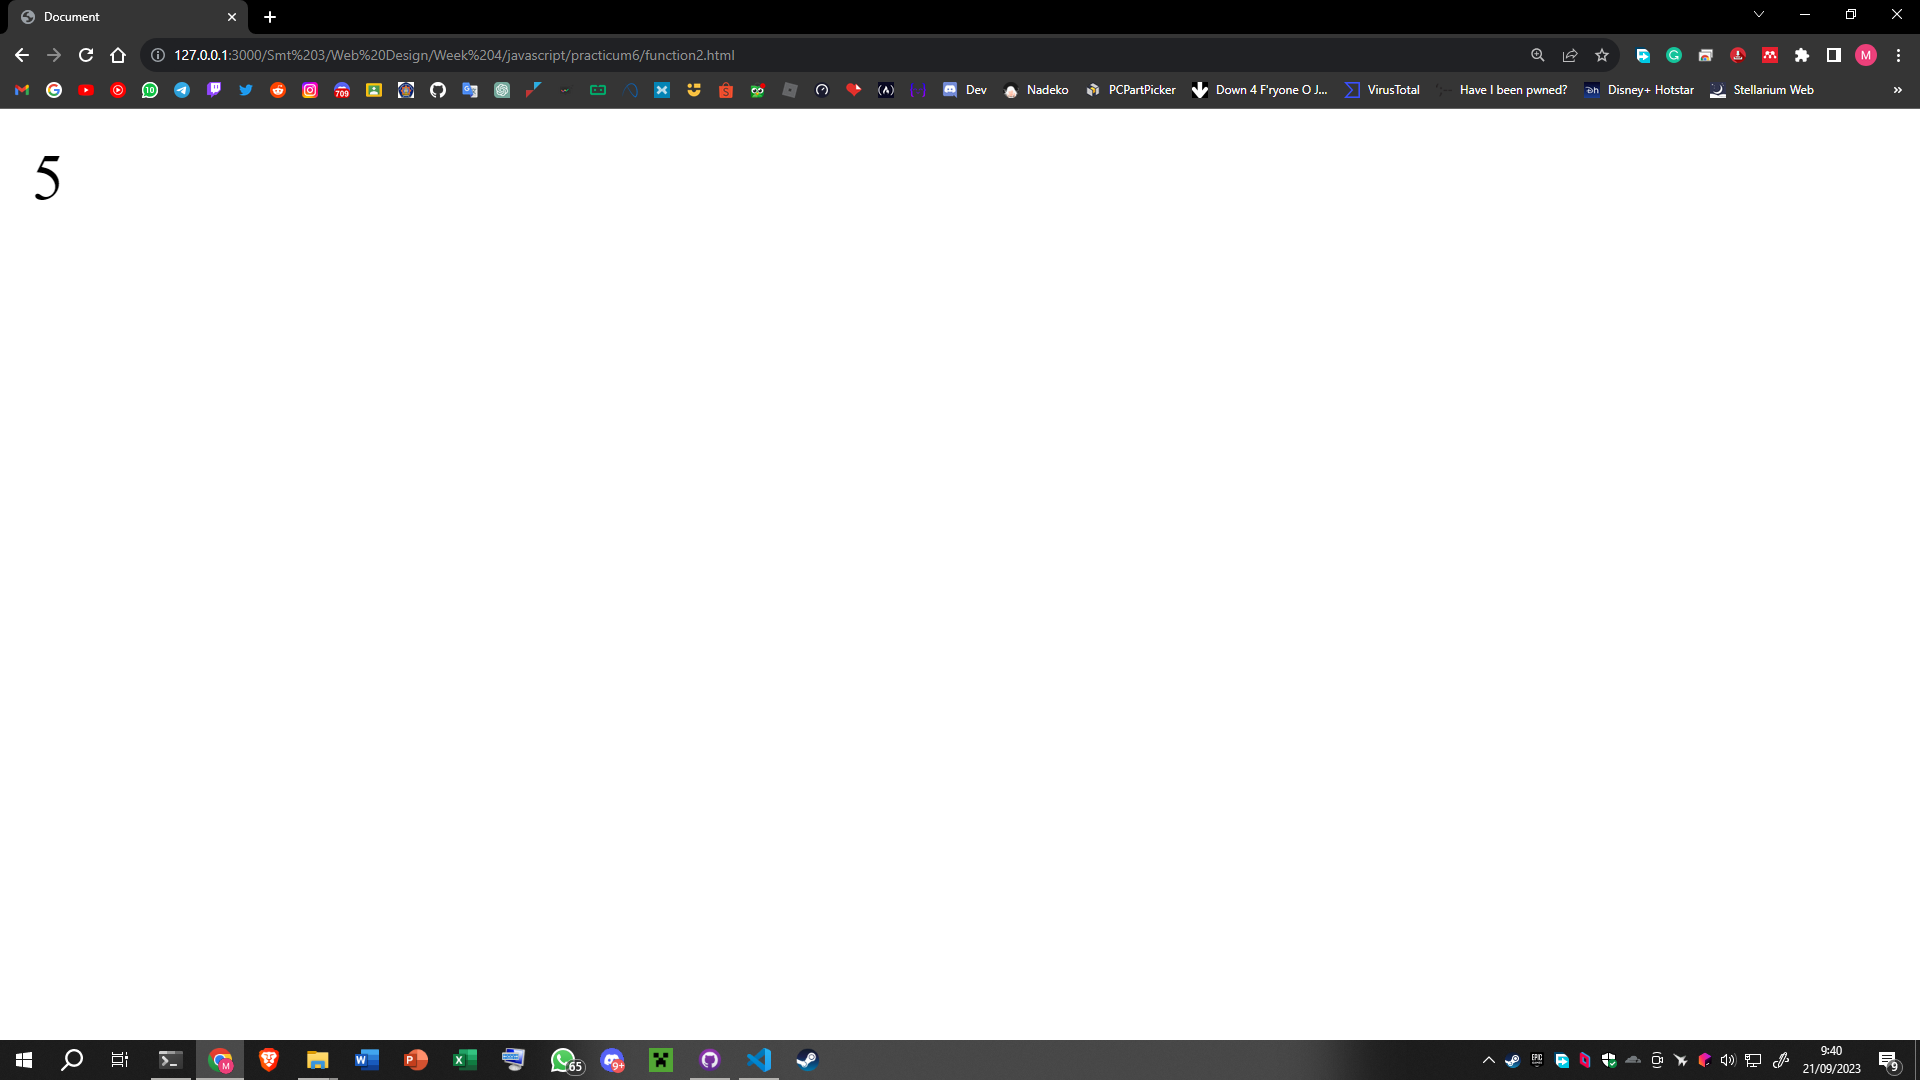
\includegraphics[width=.9\textwidth]{images/figures/fig12.png}
    \begin{minted}[autogobble,breaklines]{php}
        <?php
        function showTieredMenu(array $menu) {
            echo "<ul>";
            foreach ($menu as $key => $item) {
                echo"<li>{$item['name']}</li>";
                if (array_key_exists('subMenu', $item)) {
                    showTieredMenu($item['subMenu']);
                }
            }
            echo "</ul>";
        }
        
        showTieredMenu($menu);
        ?>
    \end{minted}
    
    \newpage

    \item - \\ \includegraphics[width=.85\textwidth]{images/figures/fig13.png} \\ The are muultiple function that can be used to manipulate string
    \item - \\ \includegraphics[width=.85\textwidth]{images/figures/fig14.png}
    \begin{enumerate}[label=\alph*.]
        \item The double quote mark will always interpreted new line escape string as a new line.
        \item While the single quotation mark will take things too literal.
        \item Here is the same case as point a.
        \item Here is the same case as point b.
        \item This case is similar to point a. but it is an example of indent escape string
        \item This case is similar to point b. but it is an example of indent escape string not being recognize.
        \item Here is an escape string meant to give clarity to the code that the part with $\backslash$" is a literal double quotation mark string.
        \item This is a simalar case to point g. but it is protrayed in single quotation mark for string with single quotation mark.
    \end{enumerate}
    
    \newpage

    \item - \\ 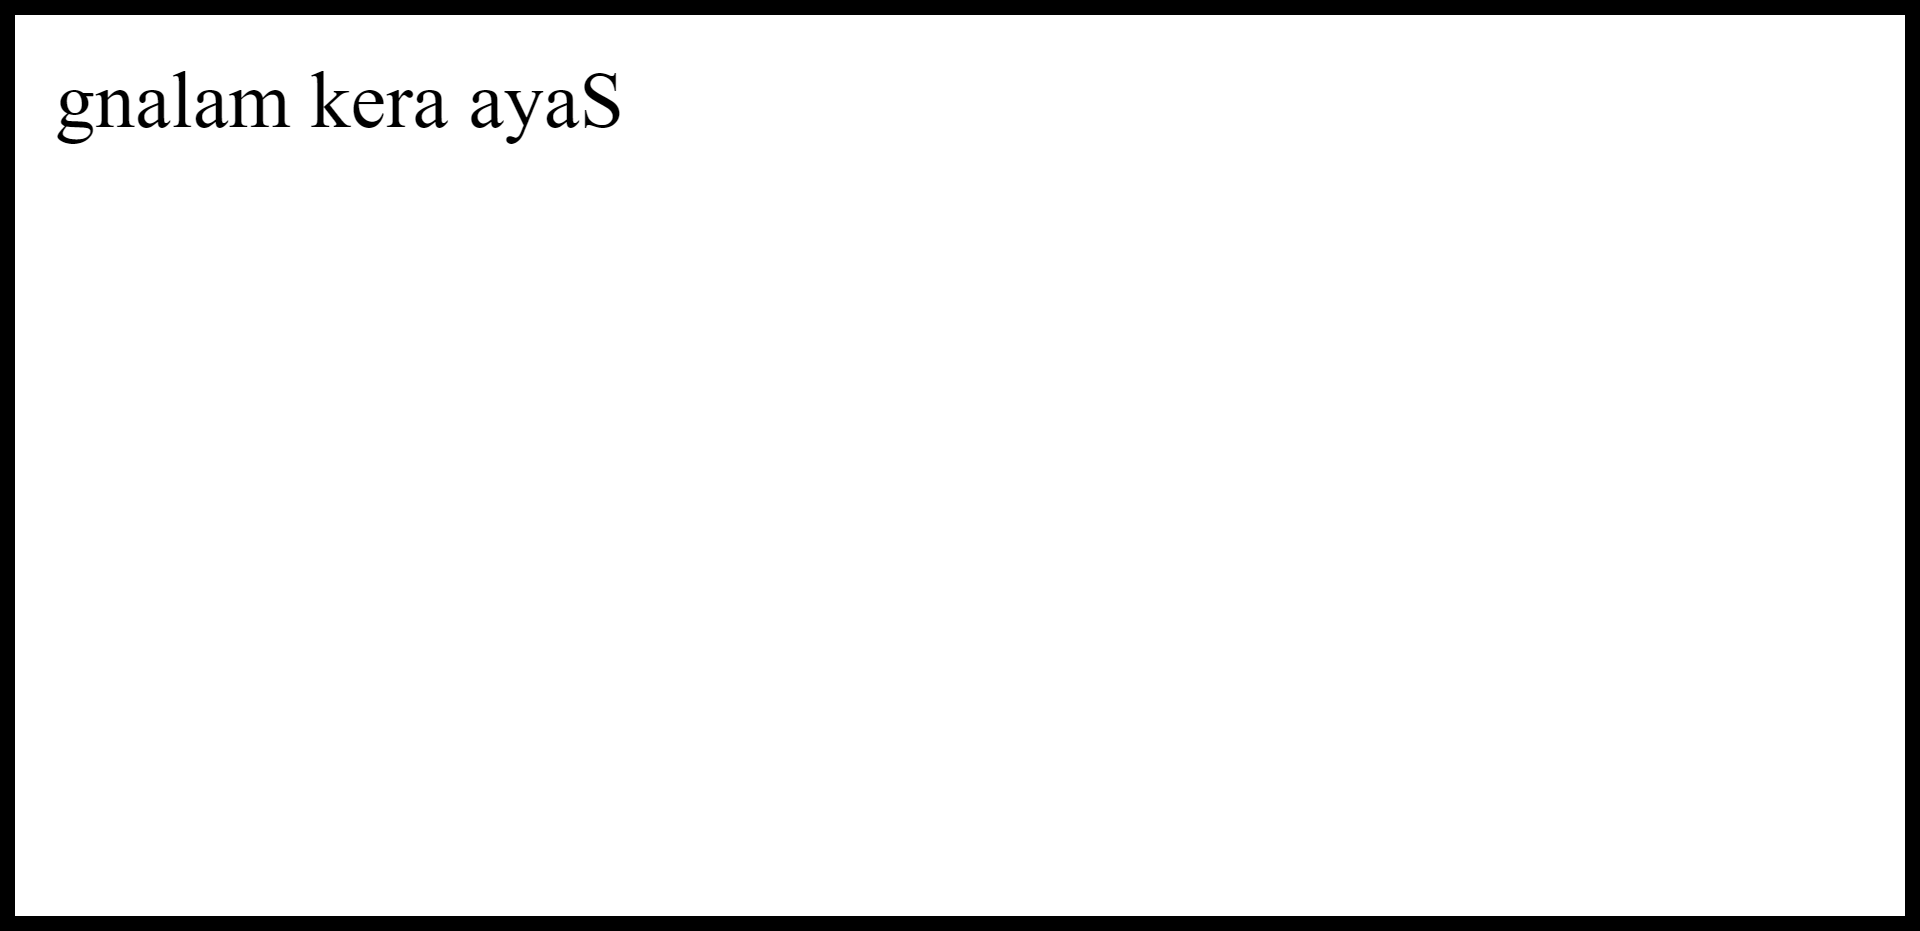
\includegraphics[width=.9\textwidth]{images/figures/fig15.png} \\ The message string is reversed
    \item - \\ \includegraphics[width=.9\textwidth]{images/figures/fig16.png} \\ The message string is reversed but with out reversing the sequence of the word
    
    \newpage

    \item - \\ 
\includegraphics[width=.9\textwidth]{images/figures/fig17.png} \\ In my opinion, it is easier to write PHP inside HTML rather than HTML in PHP because it is harder to "write" HTML syntax inside PHP
    \item - \\ \includegraphics[width=.9\textwidth]{images/figures/fig18.png} \\ HTML entities with number is more reliable than entities name
    
    \newpage
    
\end{enumerate}

\end{document}